%% FullCourse_10Lecs -- Lecture 7, Topic 7.3b: Limitations + Transition to RAG
%% Source: ./archive_pre_split/Lec07_LLM.tex (sections 9-10)
%% Pass B: layer in refinements from
%%         ../../MiniCourse_8hr/Slides/Module3_LLM_Text/M3_T3b_LLM_Limits_Measurement.tex

%% Shared preamble for the FullCourse_10Lecs topic decks.
%%
%% Each topic .tex \input's this file, then defines its own \title, \date
%% override (if any), \graphicspath, and \begin{document}.
%%
%% Reconstructed verbatim from the inlined copy preserved in
%% Lec10_Case_Studies/Lec10_T8_Case6_DeepRamsey.tex (lines 23-190), which is
%% explicitly annotated there as "from ../shared_preamble.tex, copied verbatim".
%% Base preamble matches MiniCourse_8hr/Slides/shared_preamble.tex; this version
%% additionally provides \sectiondivider, the conceptbox/cautionbox/examplebox/
%% takeawaybox tcolorboxes, and \compacttables used across the split decks.

\documentclass[10pt,english,aspectratio=169]{beamer}

\usepackage{ae,aecompl}
\usepackage[T1]{fontenc}
\usepackage{textcomp}
\usepackage[utf8]{inputenc}
\usepackage{babel}
\usepackage{datetime2}

\setcounter{secnumdepth}{3}
\setcounter{tocdepth}{3}

\usepackage{amsmath, amssymb, amsthm, graphicx}
\usepackage{booktabs, multirow}
\usepackage{tikz}
\usepackage{pgfplots}
\pgfplotsset{compat=1.16}
\usepackage[most]{tcolorbox}
\tcbuselibrary{skins, breakable, theorems}
\usepackage{listings}
\usepackage{xcolor}

\lstset{
  basicstyle=\ttfamily\small,
  keywordstyle=\color{blue!80!black}\bfseries,
  commentstyle=\color{green!50!black}\itshape,
  stringstyle=\color{orange!80!black},
  backgroundcolor=\color{gray!8},
  frame=single,
  rulecolor=\color{gray!40},
  breaklines=true,
  showstringspaces=false,
  numbers=none,
}

\lstdefinestyle{pythonstyle}{
    language=Python,
    basicstyle=\ttfamily\footnotesize,
    keywordstyle=\color{blue!80!black}\bfseries,
    commentstyle=\color{green!50!black}\itshape,
    stringstyle=\color{orange!80!black},
    frame=single,
    breaklines=true,
    showstringspaces=false,
    numbers=left,
    numbersep=5pt,
    numberstyle=\tiny\color{gray},
    backgroundcolor=\color{gray!8},
    rulecolor=\color{gray!40}
}

\ifx\hypersetup\undefined
  \AtBeginDocument{%
    \hypersetup{bookmarks=false,breaklinks=true,pdfborder={0 0 0},colorlinks=true,
      linkcolor=DarkText,urlcolor=RedTitle}%
  }
\else
  \hypersetup{bookmarks=false,breaklinks=true,pdfborder={0 0 0},colorlinks=true,
    linkcolor=DarkText,urlcolor=RedTitle}%
\fi

\makeatletter
\newcommand\makebeamertitle{%
  \begin{frame}[plain]
    \vspace*{1.0cm}
    \centering
    {\usebeamerfont{title}\usebeamercolor[fg]{title}\inserttitle\par}
    \vspace{1.0cm}
    {\usebeamerfont{author}\usebeamercolor[fg]{author}\insertauthor\par}
    \vspace{0.2cm}
    {\usebeamerfont{date}\usebeamercolor[fg]{date}\insertdate\par}
  \end{frame}}%
\AtBeginDocument{%
  \let\origtableofcontents=\tableofcontents
  \def\tableofcontents{\@ifnextchar[{\origtableofcontents}{\gobbletableofcontents}}
  \def\gobbletableofcontents#1{\origtableofcontents}%
}

\usetheme{metropolis}
\usefonttheme{professionalfonts}

\definecolor{LightGray}{RGB}{230,230,230}
\definecolor{RedTitle}{RGB}{0,0,200}
\definecolor{VeryLightGray}{RGB}{245,245,245}
\definecolor{DarkText}{RGB}{0,0,0}

\setbeamercolor{background canvas}{bg=white}
\setbeamercolor{title}{fg=RedTitle}
\setbeamercolor{author}{fg=DarkText}
\setbeamercolor{date}{fg=DarkText}
\setbeamercolor{frametitle}{bg=VeryLightGray,fg=DarkText}
\setbeamercolor{normal text}{fg=DarkText}
\setbeamerfont{title}{size=\large}

\setbeamersize{text margin left=5mm, text margin right=5mm}
\addtobeamertemplate{frametitle}{}{\vspace{-0.5em}}
\newcommand{\reducevspace}{\vspace{-0.5cm}}

% Shared section divider and box styles for split topic decks.
\newcommand{\sectiondivider}[2]{%
\begin{frame}[plain,noframenumbering]
\begin{center}
\vfill
{\Large\textbf{#1}\par}
\vspace{0.35cm}
{\normalsize #2\par}
\vfill
\end{center}
\end{frame}
}

\newtcolorbox{conceptbox}[1][]{
  colback=blue!3,
  colframe=RedTitle!55,
  boxrule=0.35mm,
  arc=1mm,
  left=2mm,
  right=2mm,
  top=1mm,
  bottom=1mm,
  #1
}
\newtcolorbox{cautionbox}[1][]{
  colback=red!3,
  colframe=red!50!black,
  boxrule=0.35mm,
  arc=1mm,
  left=2mm,
  right=2mm,
  top=1mm,
  bottom=1mm,
  #1
}
\newtcolorbox{examplebox}[1][]{
  colback=green!3,
  colframe=green!45!black,
  boxrule=0.35mm,
  arc=1mm,
  left=2mm,
  right=2mm,
  top=1mm,
  bottom=1mm,
  #1
}
\newtcolorbox{takeawaybox}[1][]{
  colback=VeryLightGray,
  colframe=RedTitle!55,
  boxrule=0.35mm,
  arc=1mm,
  left=2mm,
  right=2mm,
  top=1mm,
  bottom=1mm,
  #1
}
\newcommand{\compacttables}{\renewcommand{\arraystretch}{1.15}}

\setbeamertemplate{navigation symbols}{}
\setbeamertemplate{footline}{%
  \hfill%
  \usebeamercolor[fg]{page number in head/foot}%
  \usebeamerfont{page number in head/foot}%
  \insertframenumber\,/\,\inserttotalframenumber\kern1em\vskip2pt%
}

\makeatother

\author{Zhigang Feng}
% "date with time": compile timestamp so each build is identifiable.
\date{\today\ \DTMcurrenttime}


\usetikzlibrary{arrows.meta, positioning, shapes.geometric, fit, backgrounds}

\graphicspath{{./pic/}{../../MiniCourse_8hr/Slides/Module3_LLM_Text/pic/}{../}}

\title[AI for Econ Research]{AI for Economic Research: Dynamic Models, Language, and Agents\\
Lecture 7.3b: LLM Limitations and Transition to RAG}

\begin{document}

\makebeamertitle

%=============================================================================
\begin{frame}{Topic 7.3b Agenda}
\begin{enumerate}
  \item \textbf{Three structural limits} --- knowledge cutoff, hallucinations, context window
  \medskip
  \item \textbf{Lost-in-the-middle \& prompt sensitivity} --- positional saliency, paraphrase robustness
  \medskip
  \item \textbf{Grounded generation preview} --- cite-then-claim contract; bridge to Lec08/Lec09
  \medskip
  \item \textbf{LLMs as measurement instruments} --- AI-exposure scores from Felten/Webb to Eloundou
  \medskip
  \item \textbf{Replication: Yin--Vu--Persico (NBER 35110, 2026)} --- when only the LLM changes, regression coefficients can flip
  \medskip
  \item \textbf{Transition to RAG} --- why retrieval-augmented generation
\end{enumerate}

\bigskip
\footnotesize\textit{Arc: T1a Why$+$Tokens $\to$ T1b Embeddings $\to$ T2a Attention $\to$ T2b Transformer $\to$ T3a Training $\to$ T3b Limits $\to$ T4 Applications.}
\end{frame}

%=============================================================================
\section{Limitations}

\begin{frame}{The Knowledge Cutoff}
\begin{itemize}
\item Every pretrained LLM is trained on a \emph{static snapshot} of text. After the snapshot ends, the model learns nothing new.

\medskip
\item Each model has a \textbf{knowledge cutoff date}. After this date:
\begin{itemize}
    \item Events are invisible to the model
    \item New papers, datasets, policy announcements simply don't exist as far as it is concerned
    \item Asking ``what happened in March 2026?'' against a model trained through 2024 will at best yield ``I don't know'' --- and at worst, a confident fabrication
\end{itemize}

\medskip
\item \textbf{Why not just retrain?}
\begin{itemize}
    \item Cost: $\$10$M--$\$100$M+ for a frontier model
    \item Time: weeks to months
    \item Energy and infrastructure constraints
    \item Practically impossible to keep ``current''
\end{itemize}

\medskip
\item This is not a bug --- it is structural. Any solution that needs \emph{fresh} information must work \emph{around} the cutoff, not against it. \textbf{This is the core motivation for Lecture 8.}
\end{itemize}
\end{frame}

\begin{frame}{Hallucination Risk}
\begin{columns}[T]
\column{0.48\textwidth}
\begin{tcolorbox}[colback=red!5, colframe=red!50!black, title=\textbf{What it looks like}]
\small
\begin{itemize}
\item Fabricated citations to papers that do not exist
\item Made-up statistics that look plausible
\item Non-existent laws, cases, article numbers
\item Subtly wrong details in otherwise correct prose
\end{itemize}
\end{tcolorbox}

\column{0.48\textwidth}
\begin{tcolorbox}[colback=green!5, colframe=green!40!black, title=\textbf{Mitigations}]
\small
\begin{itemize}
\item Require and verify citations externally
\item Use retrieval (Lec08) to ground answers in real documents
\item Use tools / code: numbers from a calculator
\item Validate a sample by hand
\item Set temperature $\tau = 0$ when measuring
\end{itemize}
\end{tcolorbox}
\end{columns}

\medskip
\small\textbf{Why does it happen?} The model is trained to produce \emph{plausible-sounding} next tokens, not \emph{true} ones. Truth is a property of the world; plausibility is a property of language.
\end{frame}

\begin{frame}{Context Window Limits}
\begin{itemize}
\item Even modern models with $100{,}000$+ token context cannot swallow arbitrarily large datasets:
\begin{itemize}
    \item A 200-page 10-K filing easily exceeds short context windows
    \item Decades of FOMC transcripts cannot be loaded at once
    \item Multi-firm or multi-country panels of textual data certainly cannot
\end{itemize}

\medskip
\item \textbf{Practical consequences:}
\begin{itemize}
    \item Long inputs must be \emph{chunked}, which can break coherence and cross-reference
    \item Important information may sit outside the window altogether
    \item Attention cost is $O(n^2)$ in the context length, so doubling $n$ quadruples compute and memory
\end{itemize}

\medskip
\item Newer architectures (sparse attention, sliding-window attention, RoPE-extension, state-space hybrids) push the limit but do not eliminate it.

\medskip
\item \textbf{Implication:} you cannot just dump ``all the data'' into a prompt. You need a way to \emph{retrieve} the relevant pieces and feed them in --- another argument for RAG.
\end{itemize}
\end{frame}

\begin{frame}{Lost in the Middle: Positional Saliency in Long Contexts}
\begin{columns}[T]
\column{0.55\textwidth}
\footnotesize
\begin{itemize}
\item \textbf{Liu, Lin, Hewitt, Paranjape, Bevilacqua, Petroni, Liang} (TACL 2024): when the relevant fact sits in the \emph{middle} of a long prompt, recall drops 20--30 percentage points relative to its position at the start or end.

\medskip
\item \textbf{U-shaped recall curve.} Across closed (GPT-3.5/4) and open (LLaMA-2, MPT) LLMs, accuracy is high when the gold passage is near the start or the end of the context window and sags in the middle --- a positional bias in attention, not random noise.

\medskip
\item \textbf{Two implications:}
\begin{itemize}
    \item \emph{Stuffing the prompt} (concatenate as much as it fits) is \textbf{not a substitute for retrieval}: padding adds noise that buries the signal.
    \item RAG (Lec08) must therefore \emph{rank} chunks, not merely retrieve them. Top-ranked chunks should be placed at the prompt's ends.
\end{itemize}

\medskip
\item \textbf{Measurement consequence.} If your prompt template lists exemplars before the target, the target's effective position changes with $|\text{exemplars}|$. Two ``identical'' annotations can disagree because the model attended differently.
\end{itemize}

\column{0.42\textwidth}
\centering
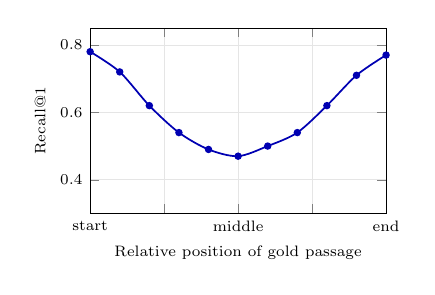
\begin{tikzpicture}[scale=0.78]
\begin{axis}[
  width=6.4cm, height=4.6cm,
  xlabel={Relative position of gold passage},
  ylabel={Recall@1},
  xmin=0, xmax=1, ymin=0.3, ymax=0.85,
  xtick={0,0.25,0.5,0.75,1.0},
  xticklabels={start,,middle,,end},
  ytick={0.4,0.6,0.8},
  grid=both,
  grid style={gray!20},
  tick label style={font=\scriptsize},
  label style={font=\scriptsize},
]
\addplot[blue!70!black, thick, smooth, mark=*, mark size=1.3pt]
  coordinates {
    (0.00, 0.78) (0.10, 0.72) (0.20, 0.62) (0.30, 0.54)
    (0.40, 0.49) (0.50, 0.47) (0.60, 0.50) (0.70, 0.54)
    (0.80, 0.62) (0.90, 0.71) (1.00, 0.77)
  };
\end{axis}
\end{tikzpicture}\\
{\scriptsize Stylized U-shape from Liu et al.\ (2024); same qualitative pattern across model families.}
\end{columns}
\end{frame}

\begin{frame}{Prompt Sensitivity --- The Same Sentence, Two Labels}
\begin{columns}[T]
\column{0.48\textwidth}
\textbf{Generic prompt:}
\begin{tcolorbox}[colback=blue!3, colframe=RedTitle!50, boxrule=0.3mm, arc=1mm, left=2mm, right=2mm, top=1mm, bottom=1mm]
\scriptsize\ttfamily
Classify this sentence:\\
"Inflation remains elevated and the Committee remains highly attentive to inflation risks."\\
Label:
\end{tcolorbox}
\smallskip
{\footnotesize Model output: \textit{neutral} --- the descriptive verbs (``remains'') and the absence of a directional action word dominate.}

\column{0.48\textwidth}
\textbf{Role-conditioned prompt:}
\begin{tcolorbox}[colback=green!3, colframe=green!45!black, boxrule=0.3mm, arc=1mm, left=2mm, right=2mm, top=1mm, bottom=1mm]
\scriptsize\ttfamily
You are a monetary economist. Is the following sentence hawkish, dovish, or neutral?\\
"Inflation remains elevated and the Committee remains highly attentive to inflation risks."\\
Label:
\end{tcolorbox}
\smallskip
{\footnotesize Model output: \textit{hawkish} --- ``highly attentive to inflation risks'' is read as a tightening signal once the prior is monetary policy.}
\end{columns}

\medskip
\footnotesize
\begin{itemize}\itemsep1pt
\item Both prompts pass the same sentence to the same model. The difference is the \emph{prior} the role + label space imposes (cf.\ ICL as Bayesian inference, T3a).
\item \textbf{Brucks \& Toubia (2025, \emph{PLOS ONE})}: primacy bias on balanced binary tasks --- GPT-4 frequently picks the \emph{first} option (a strong, robust primacy bias). Randomize option order; average across runs.
\item \textbf{WEIRD bias} \& \textbf{version drift}: training corpus is Western/English-leaning; closed-source models change silently between API calls.
\item \textbf{Take-away.} Treat the prompt as part of the research design --- freeze it, version it, report it. Robust analyses report results under multiple paraphrases.
\end{itemize}
\end{frame}

%=============================================================================
\section{LLMs as Measurement Instruments}

\begin{frame}{The Literature's Question: How Exposed Is Each Job to AI?}
\begin{itemize}
\item \textbf{The measurement problem:} map $\sim$19{,}000 O*NET tasks (or $\sim$900 SOC occupations) to a numeric \emph{AI exposure} score that can be regressed on wages, employment, and county outcomes.

\medskip
\item \textbf{Two pre-LLM generations of measures:}
\begin{enumerate}
\item \textbf{Felten, Raj, Seamans (2018, 2021)} --- AI Occupational Exposure index (AIOE). Link AI benchmark progress (image recognition, translation, $\ldots$) to O*NET ability requirements. \emph{Mechanical mapping; human raters set the abilities.}
\item \textbf{Webb (2020)} --- text overlap of AI patent abstracts with O*NET task descriptions. \emph{No raters at all --- pure TF-IDF.}
\end{enumerate}

\medskip
\item Both treat the measurement instrument as \textbf{fixed and inspectable}. A re-run next year produces the same numbers.

\medskip
\item \textbf{Economist's framing:} exposure is a \emph{measurement-error} question, not a CS question. The next slide shows what changes when the instrument is itself an LLM.
\end{itemize}
\end{frame}

\begin{frame}{Three Generations of AI-Exposure Instruments --- Compared}
\textbf{Same target (occupation-level exposure score), three very different instruments:}

\medskip
\begin{center}
\renewcommand{\arraystretch}{1.25}
\footnotesize
\begin{tabular}{|p{2.4cm}|p{3.2cm}|p{3.2cm}|p{3.2cm}|}
\hline
& \textbf{Felten, Raj, Seamans (2018, 2021)} & \textbf{Webb (2020)} & \textbf{Eloundou et al.\ (2023)} \\
\hline
Instrument & Hand-curated map: AI benchmark $\to$ O*NET ability & TF-IDF cosine: AI patent abstracts $\to$ O*NET tasks & Single LLM call: GPT-4 rates each task on 4-level rubric \\
\hline
Cost per refresh & High (human raters, weeks) & Low (re-tokenize, rerun) & Low per call; high per provider switch \\
\hline
Stability across reruns & Identical (deterministic mapping) & Identical (deterministic) & \textbf{Stochastic}; different provider $=$ different score \\
\hline
Validity assumption & Benchmark progress proxies real capability & AI patent text proxies AI capability & The LLM is a calibrated rater \\
\hline
Auditable by economist? & Yes (rater notes) & Yes (read the patent and the task) & Partially (rationale text); not the model weights \\
\hline
Failure mode & Benchmarks lag the frontier & Patent corpus is noisy & Version drift, hallucination, prompt sensitivity \\
\hline
\end{tabular}
\end{center}

\medskip
\textbf{The structural shift.} Felten and Webb treat the instrument as a \emph{document}; Eloundou treats it as a \emph{model call}. Documents do not drift. Model calls do --- which is what the next two frames quantify.
\end{frame}

\begin{frame}{The LLM-as-Rater Turn: Eloundou et al.\ (2023)}
\begin{itemize}
\item \textbf{Eloundou, Manning, Mishkin, Rock (2023, ``GPTs are GPTs'')} --- the first paper to use \textbf{GPT-4 itself} as the rater on the O*NET task list.

\medskip
\item \textbf{Rubric (per task):}
\begin{itemize}
\item \textbf{E0} --- no LLM speedup.
\item \textbf{E1} --- direct LLM access reduces task time by $\ge 50\%$.
\item \textbf{E2} --- speedup achievable with LLM-powered software built atop the model.
\end{itemize}

\medskip
\item \textbf{Procedure:} prompt GPT-4 with a task description, ask it to classify, repeat for $\sim$19k tasks, average within occupation $\to$ exposure score.

\medskip
\item Quickly adopted as the \emph{default} exposure measure --- Acemoglu (2024), IMF (2024), BIS, and many follow-ups all rebuild on this LLM-rated input.

\medskip
\item \textbf{The instrument is now the same kind of model as the subject of the research} --- and as Topic 7.3a established, that instrument is stochastic, hallucination-prone, and version-drifting.
\end{itemize}
\end{frame}

\begin{frame}{Replication: Yin, Vu, Persico (NBER 35110, 2026)}
\begin{columns}[T]
\column{0.50\textwidth}
\textbf{Design --- only the LLM changes:}
\begin{itemize}
\item Same Eloundou (2023) prompt and task list ($\sim$19k O*NET tasks, $\sim$900 occupations).
\item Three frontier 2026 annotators: \textbf{ChatGPT-5}, \textbf{Claude 4.5}, \textbf{Gemini 2.5}.
\item Identical decoding (low temperature, deterministic where supported); identical few-shot examples; identical aggregation to occupation-level $E_1$ means.
\item Plug the resulting exposure scores into the same downstream difference-in-differences regressions used by the labor-AI literature.
\end{itemize}

\column{0.46\textwidth}
\begin{center}
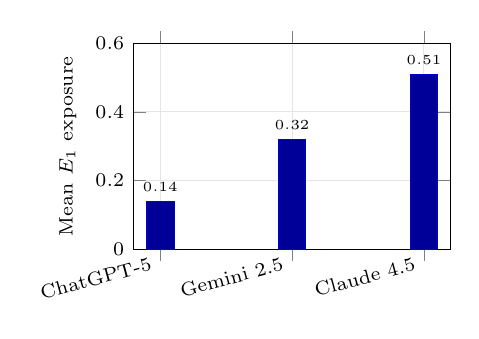
\begin{tikzpicture}
\begin{axis}[
  width=5.6cm, height=4.2cm,
  ybar,
  bar width=10pt,
  ymin=0, ymax=0.6,
  ylabel={Mean $E_1$ exposure},
  symbolic x coords={ChatGPT-5, Gemini 2.5, Claude 4.5},
  xtick=data,
  xticklabel style={font=\scriptsize, rotate=15, anchor=east},
  ytick={0,0.2,0.4,0.6},
  grid=major,
  grid style={gray!20},
  tick label style={font=\scriptsize},
  label style={font=\scriptsize},
  nodes near coords,
  nodes near coords style={font=\tiny},
]
\addplot[fill=blue!60!black, draw=blue!80!black] coordinates {
  (ChatGPT-5, 0.14)
  (Gemini 2.5, 0.32)
  (Claude 4.5, 0.51)
};
\end{axis}
\end{tikzpicture}\\
{\footnotesize Same prompt, same tasks --- 3.6$\times$ divergence in mean exposure.}
\end{center}

\smallskip
\begin{itemize}
\item \scriptsize Pairwise agreement: \textbf{56.9\%}, Cohen's $\kappa$ as low as \textbf{0.36}.
\item \scriptsize Individual DiD coefficient varies \textbf{2.4$\times$} across annotators.
\item \scriptsize County-level estimate \textbf{flips sign} (significant negative $\to$ insignificant positive).
\end{itemize}
\end{columns}

\smallskip
\textbf{What 0.36 means} (Landis--Koch benchmarks): $<\!0.20$ slight, $0.21$--$0.40$ \emph{fair}, $0.41$--$0.60$ moderate, $0.61$--$0.80$ substantial, $0.81$--$1.00$ almost perfect. Publication-grade hand-coding aims for $\kappa \ge 0.75$.
\end{frame}

\begin{frame}{Attitude in the Literature: LLMs Are Not Static Instruments}
\begin{itemize}
\item \textbf{The error is non-classical:} disagreement concentrates on tasks near the rubric boundary --- the high-exposure tasks the regressor cares about. Errors correlate with the regressor.

\medskip
\item Yin et al.: \emph{``the risks of treating evolving LLMs as static instruments.''} A paper rated with GPT-4 in 2023 cannot be re-run in 2026 and get the same labels.

\medskip
\item \textbf{Each T3b limitation $\to$ a measurement consequence:}
\begin{itemize}
\item \emph{Sampling stochasticity} $\to$ set $\tau = 0$ and report it.
\item \emph{Hallucination / mis-calibration} $\to$ ensemble across models, report Cohen's $\kappa$.
\item \emph{Version drift} $\to$ pin the snapshot; treat \emph{prompt + model + seed} as one instrument.
\end{itemize}

\medskip
\item \textbf{Emerging best practice:} pre-register prompt + model + decoding; use multiple frontier annotators and report between-model agreement; audit against a hand-coded gold standard (Topic 7.4); report inter-annotator sensitivity, not a single point estimate.

\medskip
\item \textbf{Takeaway:} the LLM is a measurement instrument --- calibrate, version, and disclose.
\end{itemize}
\end{frame}

\begin{frame}{When NOT to Use an LLM Rater --- A Decision Rule}
\textbf{Pearson 0.6 from 50 lines of \texttt{re.findall} is a real signal.} The LLM rater must clear a meaningful bar to justify its cost.

\medskip
\small
\textbf{A defensible workflow before reaching for an LLM:}
\begin{enumerate}\itemsep1pt
  \item \textbf{Hand-code 100--200 task gold standard} (you, an RA, two coders for $\kappa$).
  \item \textbf{Fit a simple baseline} --- TF-IDF + logistic regression, or a keyword rule with handful of features. Report $\kappa$ vs.\ gold.
  \item \textbf{Run the LLM in parallel.} Compute $\kappa$(LLM, gold) and $\kappa$(LLM, baseline).
  \item \textbf{Decide:}
  \begin{itemize}\itemsep0pt
    \item $\kappa$(LLM, gold) $\ge 0.75$ \emph{and} substantially $>$ $\kappa$(baseline, gold) $\Rightarrow$ LLM is validated; use it, disclose model + prompt.
    \item $\kappa$(LLM, gold) $< 0.60$ or $\approx \kappa$(baseline) $\Rightarrow$ ship the baseline; LLM doesn't earn the version-drift risk.
    \item Between $0.60$ and $0.75$ $\Rightarrow$ ensemble (LLM + baseline + tie-break by hand on disagreements).
  \end{itemize}
\end{enumerate}

\medskip
\textit{The LLM is one instrument among many, not a default. The Yin--Vu--Persico replication shows what you risk by skipping the audition.}
\end{frame}

%=============================================================================
\section{Transition to RAG}

\begin{frame}{Grounded Generation: The Linchpin for Lec08 and Lec09}
\begin{itemize}
\item \textbf{Why hallucinations happen.} A pretrained LLM is a \emph{parametric memory}: facts are baked into the weights, mixed with patterns, and re-emerge probabilistically through next-token sampling. Plausibility is what the loss optimizes; truth is not.

\medskip
\item \textbf{Two ways out --- both grounded:}
\begin{itemize}
    \item \textbf{Retrieve} the source text and condition the answer on it (\textbf{RAG, Lec08}). The model writes ``Brainard (2017) reports...'' \emph{after} the relevant Brainard paragraph appears in the prompt.
    \item \textbf{Call a tool} that returns ground-truth data (\textbf{agents, Lec09}). For a numeric fact, the model asks \texttt{fred\_query(UNRATE, ...)} and reads off the actual series.
\end{itemize}

\medskip
\item \textbf{The contract: ``cite, then claim.''} Any factual statement must be paired with the source the model is conditioning on --- a retrieved passage, a tool output, an attached file. Without that pairing, the statement is asserted from parametric memory and is auditable only by hand.

\medskip
\item \textbf{The big structural picture of the second half of the course:}
\[
   \underbrace{\text{LLM}}_{\text{language engine (Lec07)}}
   \;+\;\underbrace{\text{retrieval}}_{\text{grounded memory (Lec08)}}
   \;+\;\underbrace{\text{tools}}_{\text{grounded action (Lec09)}}
   \;\Rightarrow\;\text{auditable measurement.}
\]
\end{itemize}
\end{frame}

\begin{frame}{The Brain Metaphor}
An LLM is like a very capable brain that finished school on a fixed date.

\medskip
\begin{columns}[T]
\column{0.48\textwidth}
\begin{tcolorbox}[colback=green!5, colframe=green!40!black, title=\textbf{What the brain knows}]
\begin{itemize}
\item General language and reasoning
\item Broad economics, math, programming
\item Published papers up to its cutoff
\item Common patterns, idioms, code recipes
\end{itemize}
\end{tcolorbox}

\column{0.48\textwidth}
\begin{tcolorbox}[colback=red!5, colframe=red!50!black, title=\textbf{What the brain does \emph{not} know}]
\begin{itemize}
\item Anything that happened after the cutoff
\item Your private FOMC corpus
\item A specific firm's internal documents
\item This morning's data release
\item Your co-author's unpublished draft
\end{itemize}
\end{tcolorbox}
\end{columns}

\medskip
\textbf{Question:} how do we let this brain access the information on the right \emph{without} retraining it?
\end{frame}

\begin{frame}{Next Step: Extending the Brain}
\begin{itemize}
\item \textbf{Three options for adding new knowledge to an LLM:}
\begin{enumerate}
    \item \textbf{Retrain} from scratch with the new data. Effective, but expensive (\$M--\$B), slow (months), impractical for individual researchers.
    \medskip
    \item \textbf{Fine-tune} on the new data. Cheaper, but unreliable for injecting new \emph{facts} --- fine-tuning is good at changing style and behavior, less so at memorizing isolated facts.
    \medskip
    \item \textbf{Retrieve} relevant pieces at inference time and inject them into the prompt. Cheap, dynamic, and the model never has to be touched.
\end{enumerate}

\medskip
\item \textbf{Lecture 8} is dedicated to option 3: \textbf{Retrieval-Augmented Generation (RAG)}. A frozen LLM combined with a queryable external store of documents.

\medskip
\item \textbf{Lecture 9} goes one step further --- \textbf{agentic AI}, where the brain not only retrieves information but also \emph{acts}: runs code, fetches URLs, writes files, calls other tools. Claude Code is the running example.

\medskip
\item \textbf{Lecture 10} brings it all together with case studies of how economists actually use these tools today.
\end{itemize}
\end{frame}

\begin{frame}{Summary}
\begin{enumerate}
\item \textbf{Inputs:} tokenization $+$ embeddings $+$ positional encodings turn text into a sequence of vectors.
\smallskip
\item \textbf{Self-attention} is the core operation of the Transformer:
$Q,K,V$ projections $\rightarrow$ scaled dot-product scores $\rightarrow$ softmax $\rightarrow$ weighted sum of values.
\smallskip
\item \textbf{Stacking} layers (residuals, normalization, feed-forward networks) yields contextualized representations.
\smallskip
\item \textbf{Generation} is autoregressive: project the last embedding to the vocabulary, sample, append, repeat.
\smallskip
\item \textbf{Established applications:}
TF-IDF + cosine (Kogan et al.),
Word2Vec + BVAR (ECB Word2Prices, Araujo et al.),
fine-tuned RoBERTa (CentralBankRoBERTa, Pfeifer \& Marohl).
\smallskip
\item \textbf{2024--25 frontier:}
GPT-4 for Fedspeak (Hansen \& Kazinnik);
LLM embeddings for cross-sectional returns (Chen, Kelly \& Xiu);
transformer in SDF (Kelly et al.);
asset embeddings from holdings (Gabaix et al.).
\smallskip
\item \textbf{LLMs have a fixed knowledge cutoff.}
Next: extend the brain with retrieval --- \textbf{Lecture 8: RAG}.
\end{enumerate}
\end{frame}

\end{document}
